\chapter{Základné pojmy a definície}

\label{kap:definitions} % id kapitoly pre prikaz ref
\newtheorem{definition}{Definícia}[section]
\newtheorem{theorem}{Veta}[section]
\newtheorem{note}{Poznámka}[section]
\newtheorem{subdefinition}{Definícia}[subsection]
\newtheorem{subtheorem}{Veta}[subsection]
\newtheorem{subnote}{Poznámka}[subsection]

V tejto kapitole uvedieme základné pojmy a definície pri práci s útvarmi, ako aj súčasný stav danej problematiky. \\

\textit{Priamka} je objekt v konečnom geometrickom systéme, ktorý prechádza aspoň jedným bodom. \textit{Útvar} je množina bodov, ktoré sú spojené priamkami. \textit{Prvok} je bod útvaru, ktorý má priradenú hodnotu $x$, kde $x$ je prirodzené číslo. Prvky útvaru majú priradené navzájom rôzne hodnoty. Útvar má \textit{magickú vlastnosť} ak všetky jeho priamky majú magickú vlastnosť. \\

Ak má útvar pravidelné usporiadanie, môže byť reprezentovaný maticou (priamkami budú riadky, stĺpce a prípadne diagonály danej matice) alebo neorientovaným ohodnoteným grafom.

\section{Magické útvary}
\begin{definition} Útvar je magický ak súčet prvkov na každej jeho priamke je konštantný.
\end{definition}

\subsection{Magické štvorce}
\begin{subdefinition} Magický štvorec je matica prvkov veľkosti $n \times n$, pre ktorú platí, že súčet prvkov v každom riadku, stĺpci a na oboch diagonálach je konštantný.
\end{subdefinition}

Príklad magického štvorca je na obrázku \ref{obr:fig_basic_magic_3x3}.

\begin{figure}[H]
\centerline{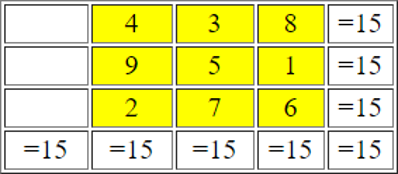
\includegraphics[width=0.3\textwidth]{images/basic_magic_3x3}}
\caption[Magický štvorec veľkosti $3 \times 3$]{Magický štvorec veľkosti $3 \times 3$ \cite{multimagie}}
\label{obr:fig_basic_magic_3x3}
\end{figure}

\begin{subnote} Ak je súčet prvkov v každom riadku a stĺpci konštantný, daný štvorec nazývame semimagickým. Ak je súčet na oboch diagonálach rovnaký, ale iný ako súčet v riadkoch a stĺpcoch, daný štvorec nazývame panmagickým.
\end{subnote}

Špeciálnu triedu tvoria magické štvorce, ktorých prvky sú $k$-tymi mocninami prirodzených čísel. Na obrázku \ref{obr:fig_squared_magic_4x4} je príklad štvorca pre $n = 4, k = 2$.

\begin{figure}[H]
\centerline{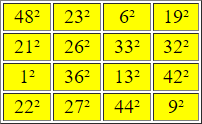
\includegraphics[width=0.3\textwidth]{images/squared_magic_4x4}}
\caption[Magický štvorec veľkosti $4 \times 4$ s druhými mocninami]{Magický štvorec veľkosti $4 \times 4$ s druhými mocninami \cite{multimagie}}
\label{obr:fig_squared_magic_4x4}
\end{figure}

Existencia štvorca pre $n = 3, k = 2$ je otvoreným problémom. Je dokázané, že ak by taký štvorec existoval, jeho prvky by museli byť vačšie ako $10^16$. Nikomu sa nepodarilo nájsť ani magický štvorec, ktorého $8$ prvkov sú druhé mocniny prirodzených čísel. A je známe iba jedno základné riešenie so $7$ prvkami (obrázok \ref{obr:fig_bremner_magic_3x3}, \cite{multimagie}), ktoré objavil v roku 1999 Andrew Bremner.

\begin{figure}[H]
\centerline{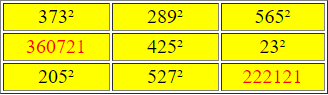
\includegraphics[width=0.4\textwidth]{images/bremner_magic_3x3}}
\caption[Magický štvorec veľkosti $3 \times 3$ so $7$ druhými mocninami]{Jediný známy magický štvorec veľkosti $3 \times 3$ so $7$ druhými mocninami \cite{multimagie}}
\label{obr:fig_bremner_magic_3x3}
\end{figure}

\begin{subnote} Existujú vzorce, ktoré dokážu vygenerovať magický štvorec so $6$ prvkami, ktoré sú druhými mocninami prirodzených čísel.
\end{subnote}

Pre $n = k = 3$ je dokázané, že taký magický štvorec neexistuje. Existencia štvorcov pre $4 \leq n \leq 6, k = 3$ je otvoreným problémom. Sébastien Miquel našiel v roku 2015 riešenie (obrázok \ref{obr:fig_miquel_magic_7x7}, \cite{multimagie}) pre $n = 7, k = 3$.

\begin{figure}[H]
\centerline{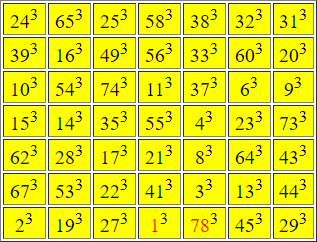
\includegraphics[width=0.4\textwidth]{images/miquel_magic_7x7}}
\caption[Magický štvorec veľkosti $7 \times 7$ s tretími mocninami]{Magický štvorec veľkosti $7 \times 7$ s tretími mocninami \cite{multimagie}}
\label{obr:fig_miquel_magic_7x7}
\end{figure}

Pre $4 \leq n \leq 10, k \geq 4$ sú známe iba semimagické štvorce \cite{multimagie}. \\

\subsection{Magické obdĺžniky}
\begin{subdefinition} Magický obdĺžnik je matica prvkov veľkosti $m \times n$, pre ktorú platí, že súčet prvkov v každom riadku je konštantný a zároveň súčet prvkov v každom stĺpci je konštantný.
\end{subdefinition}

Príklad magického obdĺžnika je na obrázku \ref{obr:fig_trenkler_magic_2x4}.

\begin{figure}[H]
\centerline{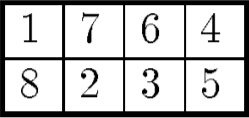
\includegraphics[width=0.2\textwidth]{images/trenkler_magic_2x4}}
\caption[Magický obdĺžnik veľkosti $2 \times 4$]{Magický obdĺžnik veľkosti $2 \times 4$ \cite{rectangles}}
\label{obr:fig_trenkler_magic_2x4}
\end{figure}

Nevyžadujeme, aby boli súčty v riadkoch a stĺpcoch rovnaké, pretože pre $m \neq n$ vieme ľahko odvodiť, že by museli byť rovné $0$ (čo je spor s tým, že prvky sú navzájom rôzne prirodzené čísla). \\

Slovenský matematik Marián Trenkler skúmal obdĺžniky veľkosti $m \times n$, ktoré sú supermagické (ich prvkami sú čísla od $1$ po $mn$) \cite{rectangles}.

\begin{subtheorem} (Trenkler, 1999) Pre všetky prirodzené $n > 2$ vieme zostrojiť supermagický obdĺžnik veľkosti $2 \times (2n - 2)$ aj $n \times n^2$.
\end{subtheorem}

Keďže obdĺžniková matica nemá diagonály, pri definícii ich neuvažujeme. Z toho vyplýva, že v ľubovoľnom magickom obdĺžniku vieme vymeniť dva riadky alebo stĺpce a magická vlastnosť ostane zachovaná. \\

Semimagické štvorce sú špeciálnym prípadom magických obdĺžnikov pre $m = n$. \\

\subsection{Magické grafy}
\begin{subdefinition} Magický graf je neorientovaný graf s ohodnotenými hranami, v ktorom pre každý vrchol platí, že súčet hrán incidentných s ním je konštantný. Vrcholy sú považované za prvky útvaru.
\end{subdefinition}

Príklad magického grafu je na obrázku \ref{obr:fig_magic_graph}.

\begin{figure}[H]
\centerline{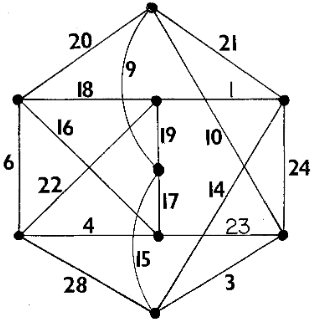
\includegraphics[width=0.4\textwidth]{images/magic_graph}}
\caption[Magický graf]{Magický graf s magickým súčtom 60 \cite{regular}}
\label{obr:fig_magic_graph}
\end{figure}

Slovenskí matematici Samuel Jezný a Marián Trenkler dokázali vetu, ktorá hovorí o tom, kedy je graf magický \cite{graphs}.

\begin{subtheorem} (Jezný, Trenkler, 1983) Graf je magický práve vtedy, keď každá hrana $G$ patrí do nejakého $(1-2)$-faktora a zároveň každá dvojica hrán $e_1, e_2$ je separovateľná $(1-2)$-faktorom grafu $G$.
\end{subtheorem}

\begin{subnote} $(1-2)$-faktor grafu je jeho rozklad na izolované hrany a kružnice.
\end{subnote} 

Na grafoch sa dajú skúmať aj iné magické vlastnosti. Môžeme ohodnotiť vrcholy a pre každú hranu zrátať súčet hodnôt jej koncových vrcholov. Alebo pre každý vrchol zrátať súčet hodnôt jeho susedov. Ku grafom vieme hľadať ich elegantné označenie (\textit{graceful labelling}).

\begin{subdefinition}
Nech $G$ je graf s $n$ vrcholmi. Elegantné označenie grafu $G$ je také priradenie hodnôt $0, ... , n-1$ jeho vrcholom, že rozdiely hodnôt susedných vrcholov sú navzájom rôzne.
\end{subdefinition}

Je dokázané, že niektoré špeciálne typy grafov ako kolesá alebo obdĺžnikové mriežky majú vždy elegantné označenie \cite{labelling}. Rozhodnúť, či k ľubovoľnému stromu existuje elegantné označenie, je dodnes otvoreným problémom. \\

\section{Multiplikatívne útvary}
\begin{definition} Útvar je multiplikatívny ak súčin prvkov na každej jeho priamke je konštantný.
\end{definition}

Príklad multiplikatívneho štvorca je na obrázku \ref{obr:fig_basic_mult_3x3}.

\begin{figure}[H]
\centerline{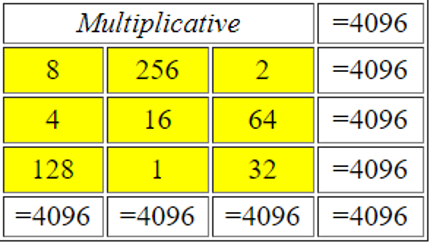
\includegraphics[width=0.3\textwidth]{images/basic_mult_3x3}}
\caption[Multiplikatívny štvorec veľkosti $3 \times 3$]{Multiplikatívny štvorec veľkosti $3 \times 3$ \cite{multimagie}}
\label{obr:fig_basic_mult_3x3}
\end{figure}

\begin{note} Semimultiplikatívne a panmultiplikatívne štvorce sú definované analogicky.
\end{note}

K ľubovoľnému magickému štvorcu vieme zostrojiť multiplikatívny štvorec napríklad tak, že všetky jeho prvky $x$ nahradíme $2^x$. \\

Tieto typy štvorcov sa dajú hľadať vzorkovou metódou. Vzorku získame tak, že zvolíme niekoľko prvkov štvorca, pričom:
\begin{itemize}
\item v každom riadku je zvolený práve jeden prvok
\item v každom stĺpci je zvolený práve jeden prvok
\item na každej diagonále je zvolený práve jeden prvok
\end{itemize}

Princíp prehľadávania je potom jednoduchý. Najprv začneme so štvorcom, ktorého všetky prvky majú hodnotu $1$. Potom si opakovane vyberieme ľubovoľnú vzorku a všetky jej zvolené prvky vynásobíme nejakou konštantou. Tým generujeme štvorec, ktorý je multiplikatívny (za predpokladu, že výsledné prvky sú navzájom rôzne). \\

\section{Bimagické útvary}
\begin{definition} Útvar je bimagický ak je magický a umocnením každého jeho prvku na druhú dostaneme opäť magický útvar.
\end{definition}

Je zrejmé, že bimagický štvorec veľkosti $2 \times 2$ neexistuje. Edouard Lucas, Luke Pebody a Jean-Claude Rosa dokázali silnejšie tvrdenia \cite{multimagie}.

\begin{theorem} (Lucas, 1891) Neexistuje bimagický štvorec veľkosti $3 \times 3$.
\end{theorem}

\begin{theorem} (Pebody, Rosa, 2004) Neexistuje bimagický štvorec veľkosti $4 \times 4$.
\end{theorem}

V roku 2006 našiel Jaroslaw Wroblewski riešenie pre $6 \times 6$ (obrázok \ref{obr:fig_wroblewski_bimagic_6x6}, \cite{multimagie}).

\begin{figure}[H]
\centerline{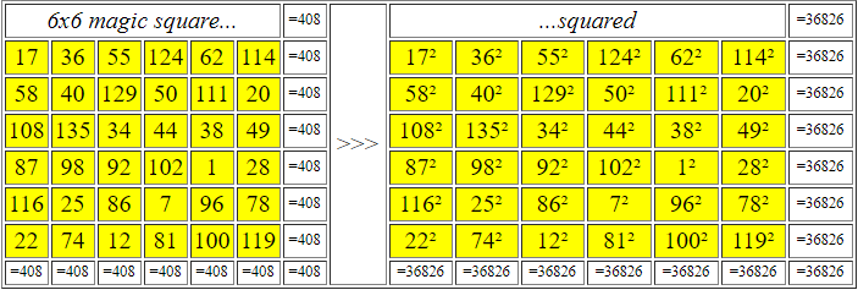
\includegraphics[width=0.7\textwidth]{images/wroblewski_bimagic_6x6}}
\caption[Bimagický štvorec veľkosti $6 \times 6$]{Bimagický štvorec veľkosti $6 \times 6$ \cite{multimagie}}
\label{obr:fig_wroblewski_bimagic_6x6}
\end{figure}

Na tomto štvorci je zaujímavé to, že má asociatívnu vlastnosť - súčet protiľahlých prvkov je konštantný. \\

Na to, aby bol štvorec veľkosti $5 \times 5$ bimagickým, muselo by byť jeho 12 magických a 12 bimagických súčtov rovnakých. Boli nájdené čiastočné riešenia, ktoré obsahovali 23 správnych súčtov \cite{multimagie}. Existencia riešenia pre $5 \times 5$ (ktoré by malo 24 správnych súčtov) je však dodnes otvoreným problémom. \\

Nasledovná veta dokazuje, že bimagických štvorcov je nekonečne veľa \cite{bimagic}:

\begin{theorem} (Chen, Li, 2004) Nech $m,n$ sú kladné celé čísla s rovnakou paritou, pričom $m,n \notin \{2,3,6\}$. Potom existuje normálny bimagický štvorec veľkosti $mn \times mn$.
\end{theorem}

Bimagické štvorce sú evidentne uzavreté na nenulový násobok. Majú však ďalšiu zaujímavú vlastnosť: sú uzavreté aj na konštantný posun. Z toho vyplýva, že vieme definovať normálne formy bimagických útvarov, ako napríklad:
\begin{itemize}
\item útvar, ktorého najmenší prvok je 1
\item útvar, ktorého magický súčet je 100
\item útvar, ktorého bimagický súčet je päťnásobkom nejakého jeho prvku
\end{itemize}

Keď predpokladáme, že bimagický štvorec je v nejakej normálnej forme, prehľadávanie sa zjednoduší. \\

\section{Multiplikatívne magické útvary}
\begin{definition} Útvar je multiplikatívny magický ak má magickú aj multiplikatívnu vlastnosť.
\end{definition}

Je zrejmé, že multiplikatívny magický štvorec veľkosti $2 \times 2$ neexistuje. Lee Morgenstern dokázal silnejšie tvrdenie \cite{multimagie}.

\begin{theorem} (Morgenstern, 2007) Neexistuje multiplikatívny magický štvorec veľkosti $3 \times 3$ ani $4 \times 4$.
\end{theorem}

V roku 2016 našiel Sébastien Miquel multiplikatívny magický štvorec veľkosti $7 \times 7$ (obrázok \ref{obr:fig_miquel_addmult_7x7}, \cite{multimagie}).

\begin{figure}[H]
\centerline{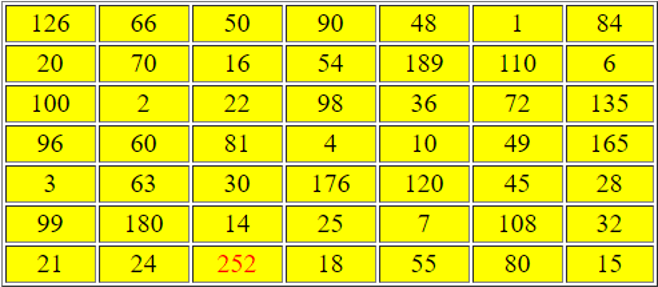
\includegraphics[width=0.5\textwidth]{images/miquel_addmult_7x7}}
\caption[Multiplikatívny magický štvorec veľkosti $7 \times 7$]{Multiplikatívny magický štvorec veľkosti $7 \times 7$ \cite{multimagie}}
\label{obr:fig_miquel_addmult_7x7}
\end{figure}

Multiplikatívne štvorce je možné nájsť napríklad vzorkovaním. Ale existencia multiplikatívneho magického štvorca veľkosti $5 \times 5$ alebo $6 \times 6$ je naďalej otvoreným problémom.











